\section{Mission}
%TODO a finir
\paragraph{Description}
L'entreprise Probespoke détenais des solutions technologiques mises en place en 2014.
Cependant une absence de suivi et de maintenance et fortement dégradé le système. L'entreprise possède deux sites vitrines, www.bgc.paris et www. probespoke.com, qui sont statiques et demande donc peu d'entretient.
Probespoke a également mis en place une application disponible sur IOs et Android relié à une plateforme ERP (entreprise resource planing). Cet plateform est construite avec le logiciel open-source odoo.
 Toutes ces solutions est sur des serveurs AWS (Amazon Web Service) dont les tarifs obscurs ont mal été compris.
\subsection{Travaux technique}
\paragraph{}
 J'ai donc du tout d'abord migrer ces serveurs d'AWS vers les serveurs d'OVH et faire ainsi passer les coûts fixes d'informatique de l'entreprise de \$1800 à \$500 .
 Pendant cette migration j'ai du également mettre la derenière version de Odoo, pour passer de Odoo 8 à Odoo 11.
 Lors de cette mise à jour des modules codés il y a quatre an se sont mis à disfonctionner, j'ai donc du en recoder une bonne partie. Finalement j'ai rajouté une fonctionnalité de prise de commande rapide sur l'application et permis sa rediffusion.
 \paragraph{}
 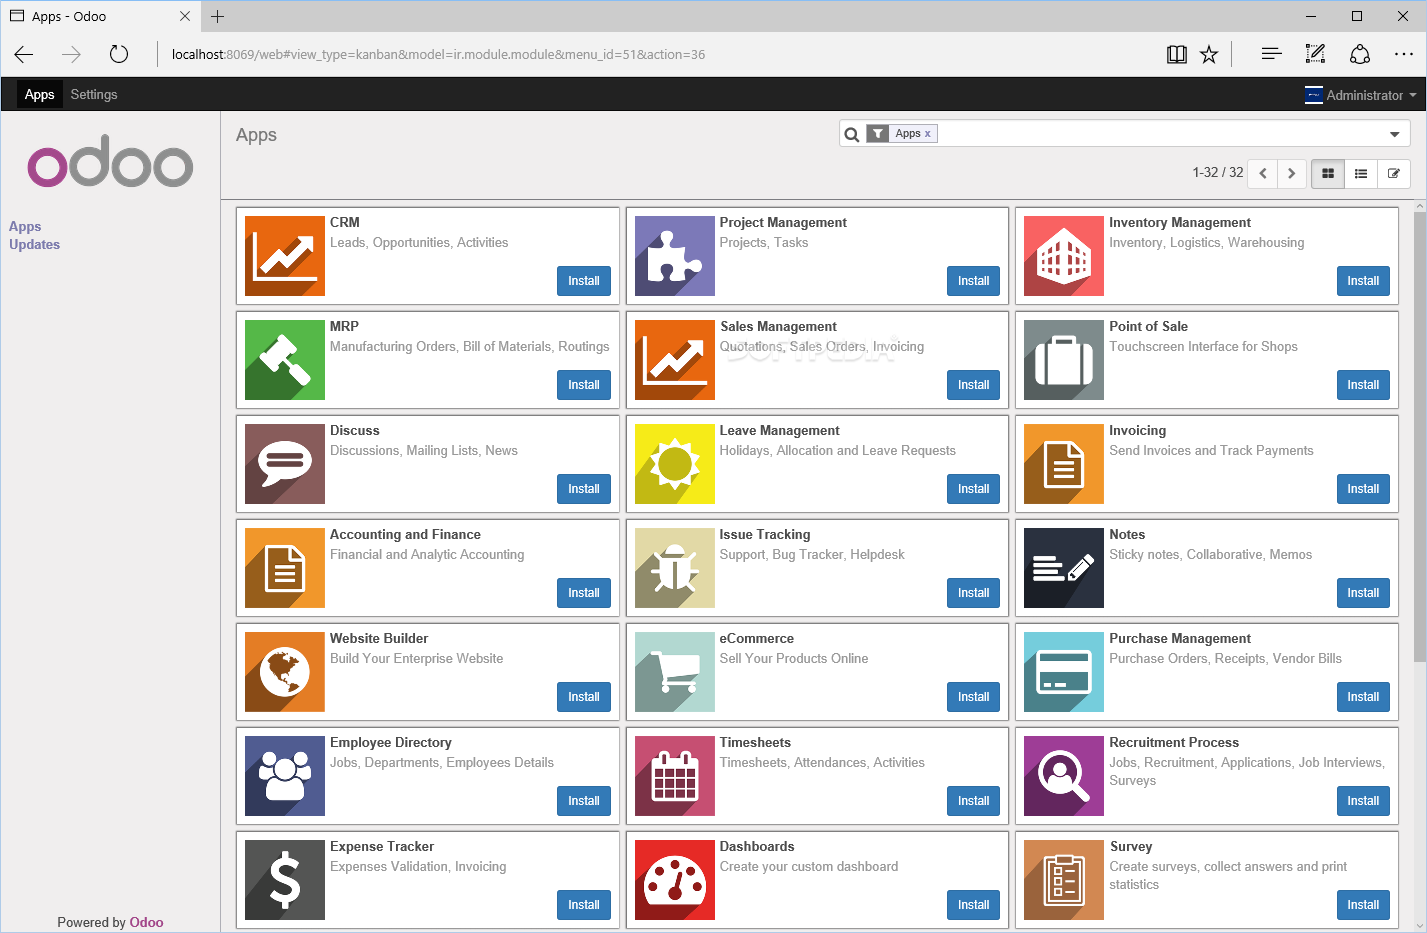
\includegraphics[width=14cm]{image/odoo.png}
 \subsection{Conseil à l'entreprise}
 \paragraph{}
 Notre employeur n'a pas pour spécialité l'informatique. Ainsi j'ai du faire des benchmarck pour trouver par exemple la solution d'hebergement de ses serveurs qui sera la moin chers. Je l'ai également mis en garde à propos de certain avancés technologiques qui le pousseront à moyen terme à une réorganisation de ses services. Finalement il m'a également été demandé d'aider à écrire une demande de devis pour poursuivre la mise en place de son système informatique. Etant pris par son rôle commerciale, notre employeur n'a peu de temps pour s'interressé aux avancés technologiques. De plus Probespoke n'engage pas d'informaticien à temps plein, ainsi les avancés dans ce domaine sont sacader. De mon points de vue celà est une erreur étant donné la place predominante de l'informatique dans cette entreprise.
 \paragraph{}
 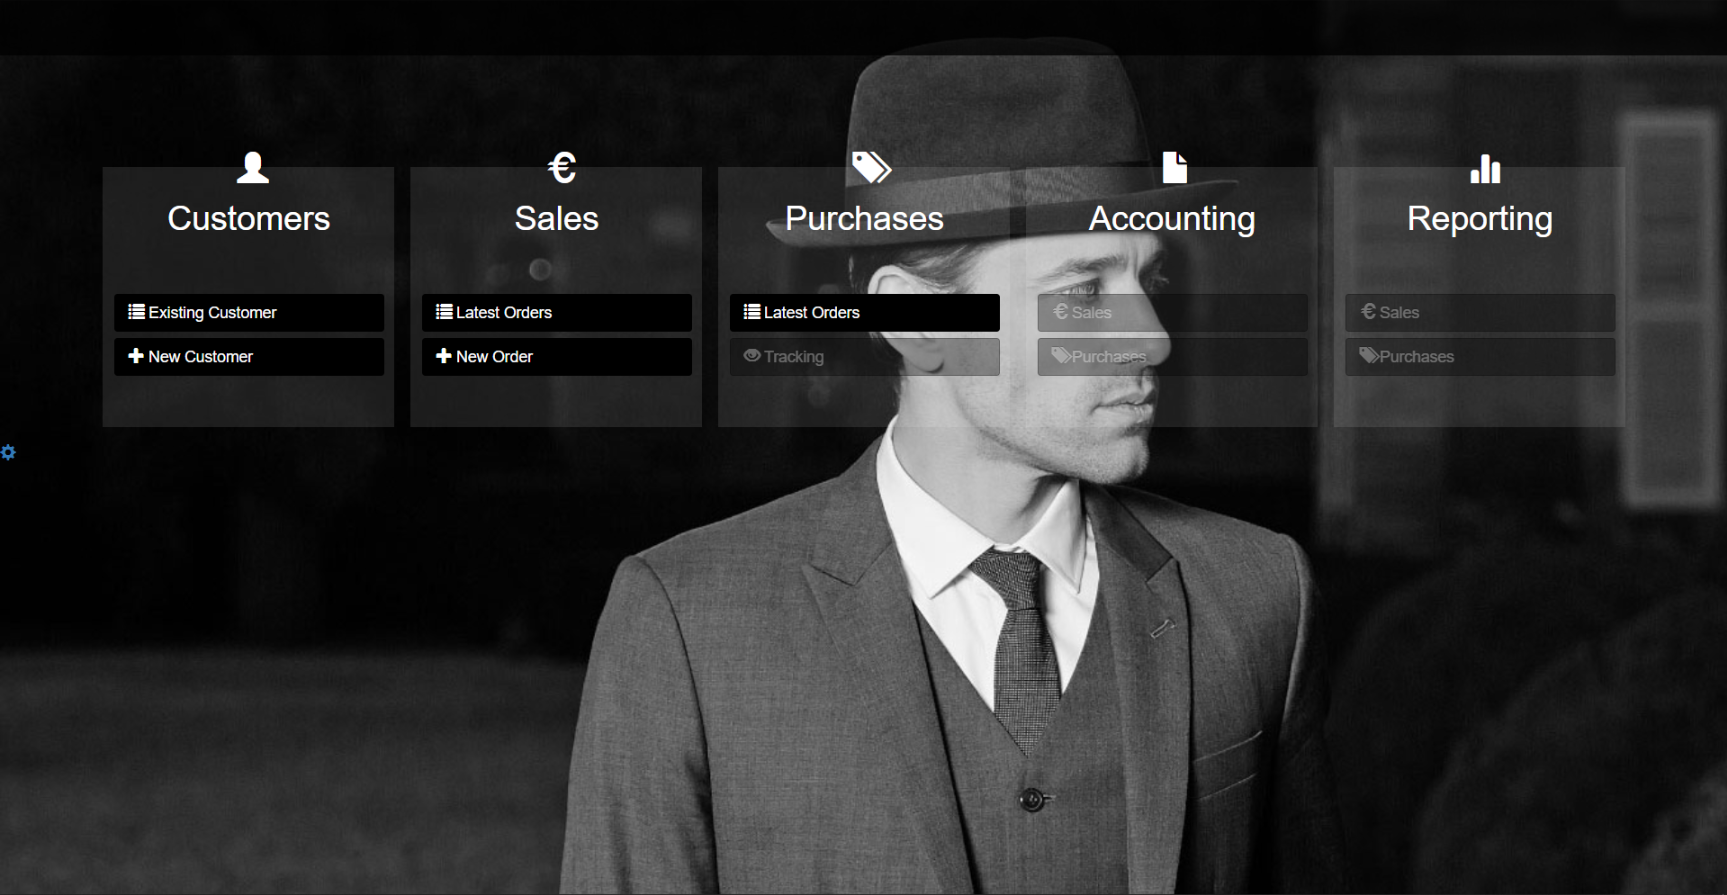
\includegraphics[width=16cm]{image/prise.png}
